\chapter{Software de adquisición}
\label{cap2}
En este capítulo procederemos a explicar el funcionamiento del software de adquisición. Empezaremos recordando los aspectos básicos descritos en el
capítulo \ref{cap1}. El software de adquisición es el encargado de coordinar la estación. El funcionamiento nominal del software consiste en recoger
la información de los demás módulos y guardar la en una base de datos. Aparte de dotarle de esta funcionalidad nominal el software debe ser capaz de
iniciarse automáticamente y recuperarse ante posibles fallos.  
\par
El software se ejecuta sobre un Linux en una placa BeagleBone Black\cite{Beagle}\cite{BeagleWiki}. El lenguaje utilizado para el desarrollo del
software es Python\cite{Python}. Para la gestión de la base de datos hemos elegido Sqlite3\cite{Sqlite}. Al ser un software para un sistema empotrado
es conveniente estar familiarizados con el entorno hardware, descrito en el capítulo \ref{entornoHW}.
\par
En la figura \ref{fig:soft_adquisición} podemos ver un diagrama de flujo que describe el funcionamiento de nuestro software. A lo largo de este
capítulo haremos muchas referencias a este diagrama para explicar los diferentes módulos software que lo componen. Podemos ver que hay 4 módulos
principales, a continuación haremos una breve descripción de estos. 

\begin{itemize}
  	\item	\texttt{NMDA}. Es el proceso principal de nuestro software. Este es el encargado de realizar las configuraciones necesarias e iniciar
	  	el \texttt{FPGASerialReader} y el \texttt{CountsManager}.
	\item	\texttt{FPGASerialReader}. Thread que se encarga de procesar la información transmitida por la FPGA.
	\item	\texttt{CountsManager}. Thread que se encarga de pedir la información necesaria y guardarla en la base de datos con periodicidad de un
	  	minuto. Después de guardar la información de un nuevo minuto este inicia el \texttt{DBUpdater}.
	\item	\texttt{DBUpdater}. Thread que se encarga de sincronizar la base de datos local con la replica remota.
\end{itemize}

\begin{sidewaysfigure}[p]
	\centering
	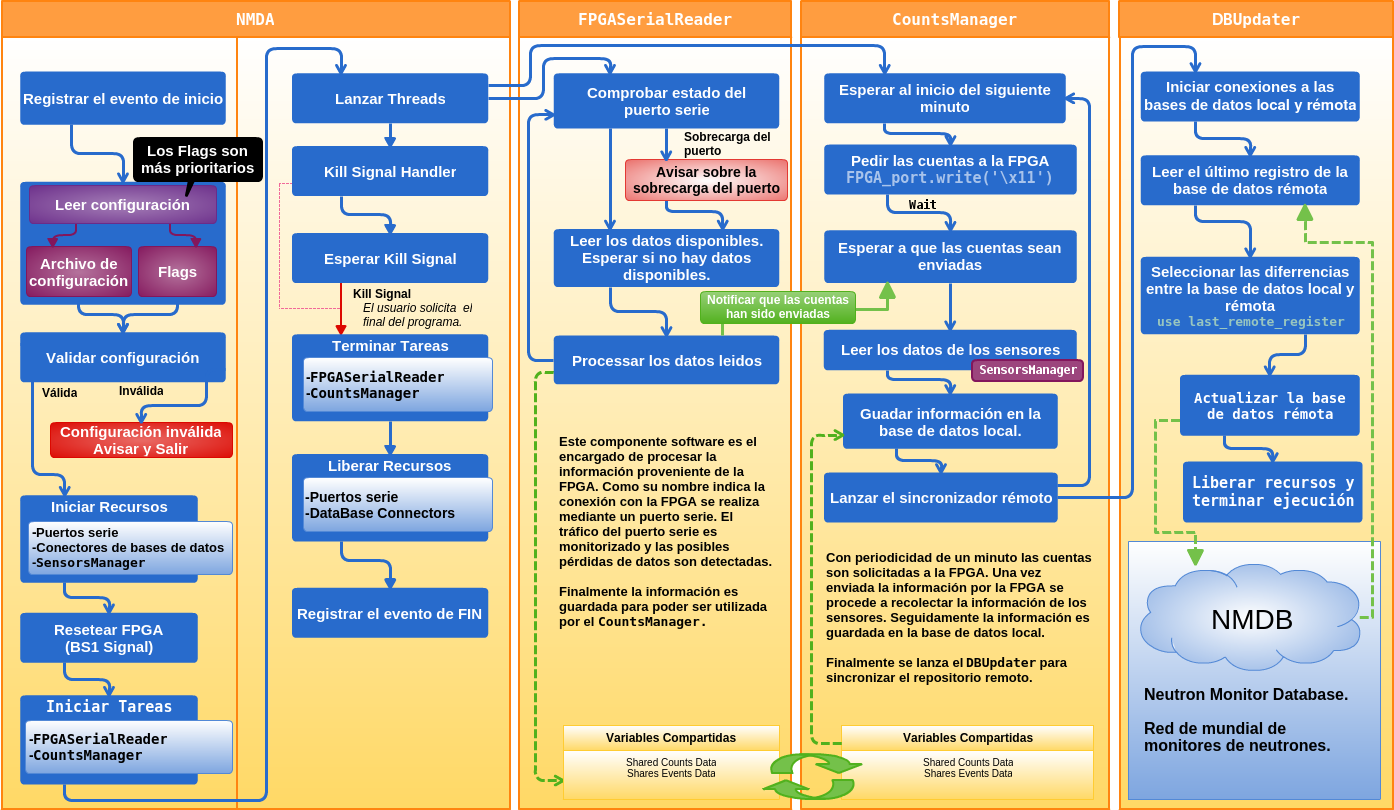
\includegraphics[keepaspectratio, width=1\textwidth]{./img/soft_adquisicion.png}
	\caption{Diagrama de flujo. Software de adquisición.}
	\label{fig:soft_adquisición}
\end{sidewaysfigure}

\section{Arranque automático del sistema}
	Uno de los requisitos del sistema es que se ponga en marcha automáticamente ante la presencia de corriente eléctrica. La BeagleBone Black por
	defecto está configurada para que arranque automáticamente. Nos queda configurar el sistema operativo para que arranque nuestro software de
	forma automática. Para este propósito vamos a utilizar las \emph{System Services}\cite{AngSystemctl} que Angstrom nos ofrece. Un servicio de
	sistema nos permite ejecutar un programa de forma automática al ser arrancado el sistema. Angstrom utiliza \texttt{systemd}\cite{systemdWiki}
	para gestionar los servicios de sistema. Este es un conjunto de demonios, librerías y utilidades diseñados para facilitar la administración de
	sistemas Linux.
	\par
	Para manejar la configuración de \texttt{systemd} tenemos el comando \texttt{systemctl}. A continuación podemos ver como usar este comando.
	\begin{lstlisting}[style=myBash]
$ systemctl start    nombre_de_servicio
$ systemctl restart  nombre_de_servicio
$ systemctl stop     nombre_de_servicio
$ systemctl status   nombre_de_servicio
$ systemctl enable   nombre_de_servicio
$ systemctl disable  nombre_de_servicio
	\end{lstlisting}
	Los servicios de sistema se crean mediante archivos con extensión \texttt{.service} que deben ser guardados en el directorio
	\texttt{/lib/systemd/system}. En el apéndice \ref{appendix:systemctl} podemos ver el contenido de los archivos que definen los cuatro
	servicios de sistema que utilizamos en este trabajo. Veamos el significado de lo campos más importantes que se definen en estos archivos.
	\begin{itemize}
		\item	\texttt{Description}. Un mensaje descriptivo del servicio. Permite al usuario entender el propósito de este de forma fácil.
		\item	\texttt{Before} y \texttt{After}. Con estos dos campos podemos referenciar a otros servicios para indicar que este servicio
		  	debe ejecutarse antes o después del servicio que es citado. Estos dos campos nos permiten definir un orden en el que serán
		  	ejecutados los servicios de sistema. También podemos especificar un grupo de servicios como el \texttt{network.target} que
			agrupa los servicios responsables de establecer una conexión Internet. 
		\item	\texttt{Type}. El tipo del servicio. Con este campo podemos dar diferentes propiedades a nuestro servicio. Los valores
		  	aceptados que nosotros utilizamos son \texttt{oneshot}, \texttt{forking} y \texttt{simple} que es el valor por defecto.
		\item	\texttt{ExecStart}. El comando y argumentos que queremos ejecutar.
		\item	\texttt{WantedBy}. Es el grupo al que este servicio pertenece. El grupo \texttt{multi-user.target} es un grupo para los
			servicios de un sistema multiusuario, un sistema no gráfico. Este campo hace que este servicio sea retrasado hacia el final
			del proceso de arranque, específicamente hasta que el sistema sea listo para aceptar la entrada de múltiples usuarios. 
	\end{itemize}
	\par
	En la figura \ref{fig:boot} podemos ver la secuencia que define el proceso de arranque del sistema de adquisición. Para cumplir con este
	proceso hemos definido cuatro servicios de sistema. El servicio \texttt{myWatchDog.service} es el encargado de arrancar el software que
	controla el Watchdog. El servicio \texttt{ntpdate.service} es el responsable de actualizar la fecha y hora actuales. El servicio
	\texttt{ntpd.service} es el responsable de mantener la fecha y hora actuales. Finalmente el servicio \texttt{nmda.service} es el encargado de
	arrancar el software de adquisición.
	\begin{figure}[h]
		\centering
		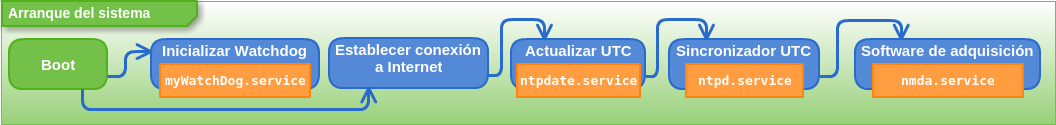
\includegraphics[keepaspectratio, width=1\textwidth]{./img/boot.png}
		\caption{Arranque del sistema}   
		\label{fig:boot}
	\end{figure}
	\subsection{Watchdog}
		Un Watchdog \cite{WatchDogWiki} es un mecanismo de seguridad que realizar un Reset en el sistema cuando se detecta un
		malfuncionamiento. Consiste en un temporizador que realiza una cuenta atrás, cuando esta cuenta llega a cero el sistema es reiniciado.
		Es nuestro software el que debe reiniciar este contador para que no expire. Los Watchdogs pueden ser software o hardware, el que
		utilizamos nosotros esta implementado en la BeagleBone Black y es hardware.
		\par
		El Watchdog es accesible mediante el archivo \texttt{/dev/watchdog}. Para activar el mecanismo escribimos en el archivo, cualquier
		valor es aceptado. El contador es puesto en marcha, si este llega a expirar es reiniciada la placa. El valor inicial del contador es
		de 60 segundos, valor que adquiere cada vez que es reiniciado. El contador es reiniciado al escribir en el archivo. Al cerrar dicho
		archivo el mecanismo es deshabilitado. A continuación presentamos una parte del código fuente responsable de controlar el WatchDog.
		\begin{lstlisting}[style=myPython]
args		= NMDA.create_parser().parse_args()
conn_local      = sqlite3.connect(args.database)
last_data       = get_last()
cont            = 0

wd = open("/dev/watchdog", "w+")
while True:
    time.sleep(20)
    wd.write("\n")
    wd.flush()
    cont+=1

    if cont >= 15:            #15*20secs=5mins
        cont            = 0
        curr_last       = get_last()
        if curr_last == last_data:
            time.sleep(120)   #Este sleep reinicia la placa
        last_data       = curr_last
		\end{lstlisting}
		Primero se establece la conexión con la base de datos local. La base de datos es utilizada para comprobar si el sistema de adquisición
		genera correctamente datos, si no son generados datos la placa debe ser reiniciada. Una vez establecida la conexión procedemos a
		invocar la función \texttt{get\_last()}, que devuelve el último valor presente en la base de datos. Seguidamente procedemos a abrir el
		archivo  que nos permite manejar el WatchDog. Una vez abierto el archivo entramos en un bucle \texttt{while} sin condición de salida.
		En cada iteración de este bucle escribimos un salto de línea que reinicia el contador del WatchDog. Dentro del bucle también tenemos
		una llamada a la función \texttt{time.sleep(20)}, las iteraciones del bucle están espaciadas 20 segundos. Cada 15 iteraciones o
		aproximadamente 5 minutos volvemos a invocar la función \texttt{get\_last()}. El valor devuelto es comparado con el valor anterior. Si
		estos dos valores son iguales invocamos la función \texttt{time.sleep(120)}, intervalo suficiente para que el contador del WatchDog
		expire. Los valores son iguales si en los últimos 5 minutos el sistema de adquisición no ha generado ningún dato. Por contrario si se
		han generado datos durante los últimos 5 minutos estos dos valores son diferentes, en tal caso se sigue con la ejecución del bucle
		\texttt{while}. 
	\subsection{Sincronización UTC}
		La BeagleBone Black no implementa ningún mecanismo hardware para calcular la fecha y hora actuales, por lo que en cada reinicio la
		fecha y hora se pierden. Es nuestra responsabilidad realizar un mecanismo software que nos sincronice con el resto del
		mundo\cite{ntpd}.  Utilizaremos el programa \texttt{ntpd} para este propósito. este es un programa que hace uso del \emph{Network Time
		Protocol}\cite{ntpWiki} para mantener el tiempo del sistema. Haremos dos llamadas a este programa.
		\begin{lstlisting}[style=myBash]
# Actualiza la fecha y hora.
$ /usr/bin/ntpd -q -g -x
# Lanza un demonio que corrige las derivas que puedan presentarse
$ /usr/bin/ntpd -p /run/ntpd.pid
		\end{lstlisting}


\section{\texttt{NMDA}}
	Este es el módulo principal de nuestro software. En la figura \ref{fig:soft_adquisición} podemos ver un diagrama de flujo que representa el
	funcionamiento de este. En las siguientes subsecciones describiremos las funcionalidades más relevantes de este módulo.
	\subsection{Logger}
		Haciendo uso de la librería \texttt{logging}\cite{py_logging} configuramos un archivo de Log. En este archivo iremos registrando eventos importantes
		que sucedan. Ejemplo de eventos que registramos son las pérdidas de datos o el inicio del sistema. El mecanismo está configurado para
		que automáticamente se guarde la hora y fecha de cada mensaje. A continuación se muestra como se configura y usa este mecanismo.
		\begin{lstlisting}[style=myPython]
import logging
logging.basicConfig(filename='/server/logs/NMDA.log', level=logging.DEBUG, format=''%(asctime)s %(message)s'')
logging.info('Started')
		\end{lstlisting}
	\subsection{Archivo de configuración y Flags}
		Existen una serie de variables que varían en función de la estación o que simplemente pueden cambiar con el tiempo. No es buena idea
		tener los valores de estas variables en el código. Este problema nos ha llevado a exportar estas variables a un archivo de configuración.
		Para leer este archivo utilizamos la librería \texttt{ConfigParser}\cite{py_ConfigParser}. A continuación mostramos un ejemplo de este
		archivo que nos ayudara a entender mejor su estructura.
		\begin{lstlisting}[style=myFile]
[Basics]
# The serial RS232_FPGA1C
serial_port_control  = /dev/ttyO2
# The local database where data will be saved. If 'shell' is specified as database data will be printed to the shell
database = /server/data/test.db
# Channel averages used for the median algorithm\ldots
Channel_avg = 255, 290, 0, 295, 0, 0, 289, 291, 252, 254, 293, 299, 298, 328, 299, 302, 302, 272

[Sensors]
# The serial RS232_FPGA1
serial_port_sensors= None
# The type of barometer that will be used. 'None', 'bm35', 'ap1'
barometer_type = None
# The type of hvps that will be used. 'None', 'analog', 'digital'
hvps_type = None
#Correction coefficient for the analog hvps, 1.0 => No correction
analog_hvps_corr = 1.0

[dbUpdater]
db_updater_enabled=True
# Must be the same that Basic.database
local_db= /server/data/test.db 
# The remote database config
remote_db_host= 192.168.1.1
# The user must have privileges
remote_db_user= hristo
remote_db_pass= 123qwe
# The database will be created if not exists along with all the tables
remote_db_db= nmdadb2

[Pressure]
# Average pressure for the station.
avg_pressure=932
# N=N0*exp(Beta*(P-P0))
beta_pressure=0.0067

[Efficiency]
# corr_efficcincy = Beta * corr_pressure
beta_efficiency=1.0
\end{lstlisting}
		Los valores de las variables exportadas son también accesibles mediante el uso de Flags. En este caso hemos utilizado la librería 
		\texttt{argparse}\cite{py_argparse}. Los valores que son especificados con Flags sobrescriben a los valores del archivo de
		configuración. Los Flags se usan de la siguiente forma.
		\begin{lstlisting}[style=myBash]
$ python NMDA.py -h
usage: NMDA.py 
   [-h] [-sp SERIAL_PORT_CONTROL] [-db DATABASE]
   [-sps SERIAL_PORT_SENSORS] [-bm {ap1,bm35}]
   [-hv {digital,analog}] [-ahvc ANALOG_HVPS_CORR]
   [-dbU DB_UPDATER_ENABLED] [-ldb LOCAL_DB] [-rh REMOTE_DB_HOST]
   [-ru REMOTE_DB_USER] [-rp REMOTE_DB_PASS] [-rdb REMOTE_DB_DB]
   [-apr AVG_PRESSURE]
		\end{lstlisting}
	\subsection{Iniciar recursos}
		Al ser el módulo principal, \texttt{NMDA} es el encargado de iniciar todos los recursos que serán utilizados. Por recursos nos
		referimos a las variables compartidas, conectores a las bases de datos, interfaces de los puertos serie y otros. Lo más interesante de
		este apartado es que las tablas de las bases de datos son creadas automáticamente si no existen. Esto simplifica mucho la tarea de
		implantar el software.
	\subsection{Resetear FPGA}
		Como hemos explicado en el capítulo \ref{entornoHW} la FPGA nos permite realizar un Reset, nuestro software realizara uno antes de
		empezar con la adquisición de datos. Este Reset nos asegura que la FPGA estará en un correcto estado. Para realizar el Reset de la
		FPGA utilizaremos la entrada digital que está conectada al pin \emph{P9\_42} de la BeagleBone Black. Volvemos a recordar que la señal
		digital es activa a nivel bajo. Para controlarla utilizaremos la librería de \emph{AdaFruit}\cite{AdaFruitGit} de la siguiente manera.
		\begin{lstlisting}[style=myPython]
import Adafruit_BBIO.GPIO as GPIO
GPIO.setup('P9_42', GPIO.OUT)
GPIO.output('P9_42', GPIO.LOW)
time.sleep(0.5)
GPIO.output('P9_42', GPIO.HIGH)
		\end{lstlisting}
	\subsection{Iniciar Tareas}
		El siguiente paso es iniciar los dos Threads, \texttt{CountsManager} y \texttt{FPGASerialReader}. Son estos dos Threads los que
		realizan todo el proceso de adquisición, serán descritos más adelante en este capítulo. 
	\subsection{Kill Signal Handler}
		Este es un software que debe ejecutarse indefinidamente. En su uso real no será interrumpido, pero hemos implementado un mecanismo que
		nos permite pararlo. Este mecanismo nos permite solicitar el fin del programa, que desencadena una serie de acciones. Estas acciones
		tienen como objetivo asegurar que todos los recursos sean liberados de forma correcta. Liberar los recursos de forma correcta supone
		no tener ningún conflicto si seguidamente volvemos a ejecutar el software. Esto en el uso real del software no tiene gran impacto, sin
		embargo ha sido muy útil en el proceso de desarrollo.

\section{\texttt{FPGASerialReader}}
	Este módulo software es el encargado de leer y procesar los datos transmitidos por la FPGA. En la figura \ref{fig:soft_adquisición} podemos
	ver un diagrama de flujo que refleja el funcionamiento de este. La ejecución del Thread empieza comprobando el estado del puerto serie, que
	puede estar saturándose. En el caso de que el puerto se esté saturando es generada una estrada en el archivo de Log. A continuación leemos
	los datos disponibles, en caso de no haber datos disponibles el Thread se queda bloqueado esperando a la llegada de estos. Seguidamente de
	leer los datos pasamos a procesar los, por procesar nos referimos a interpretar el significado que tienen. Finalmente volvemos al paso inicial.  
	\par
	En las tablas del capítulo \ref{entornoHW} podemos ver el formato de los datos que tenemos que procesar. Vemos que hay tres tipos de mensajes
	que podemos recibir. Los mensajes no siguen un orden concreto, además llegan de forma totalmente asíncrona. Los mensajes son transmitidos en
	forma de bytes. El canal de transmisión no asegura la correcta transmisión de los bytes por lo que algunos se pueden perder. Todo esto
	conlleva a que procesar los datos no sea tarea fácil.
	\par
	Para este propósito hemos implementado una máquina de Moore. Si nos volvemos a fijar en el formato de los datos podemos ver que los primeros
	bits de cada byte son fijos. Estos bits nos ayudan a identificar a que mensaje corresponde el byte. Los estados y transiciones de la maquina
	pueden verse en la figura \ref{fig:reader}. El estado inicial es \texttt{ByteX}. Aunque no esté reflejado en la figura la recepción de cualquier
	valor no esperado nos lleva al estado inicial.
	\par
	La información generada al procesar los datos es almacenada en las variables compartidas. Estas variables son accesibles desde el 
	\texttt{CountsManager}.
	\begin{figure}[h]
		\centering
		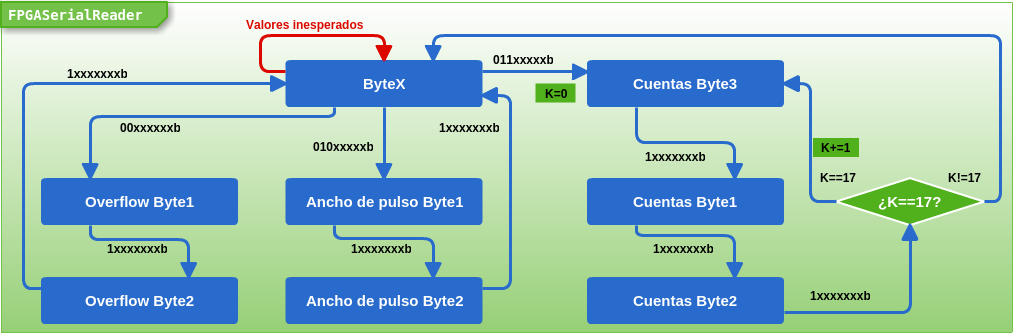
\includegraphics[keepaspectratio, width=1\textwidth]{./img/reader.png}
		\caption{Máquina de Moore. \texttt{FPGASerialReader}.}   
		\label{fig:reader}
	\end{figure}

\section{\texttt{CountsManager}}
	Este es el módulo software encargado de recolectar la información de los demás módulos y guardarla en una base de datos. En la figura 
	\ref{fig:soft_adquisición} podemos ver el diagrama que describe el funcionamiento de este. La mayoría de los datos que este módulo maneja son
	generados por los otros módulos software como el \texttt{FPGASerialReader} o el \texttt{SensorsManager}, este tan solo calcula el valor global
	y las correcciones de este. Finalmente este se encarga de guardar los datos. 
	\subsection{Solicitar cuentas a la FPGA}
		Como vimos en el capítulo \ref{entornoHW} la FPGA tan solo transmite los datos de las cuentas cuando estas son solicitadas con el
		comando apropiado. Este módulo es el encargado de mandar el comando al principio de cada minuto. La información transmitida por la
		FPGA es procesada por el \texttt{FPGASerialReader} y almacenada en variables compartidas accesibles por el \texttt{CountsManager}.
		Después de mandar el comando apropiado para solicitar las cuentas este Thread se queda esperando hasta que el \texttt{FPGASerialReader}
		le notifique de que las cuentas han sido enviadas y procesadas. Al ser notificado este módulo procede a leer de las variables
		compartidas donde está almacenada la información de las cuentas.
	\subsection{Median Algorithm y Correcciones}
		Como hemos comentado al principio de esta sección este módulo calcula el valor global y una serie de correcciones sobre este. El valor
		global es una representación de las mediciones de todos los tubos, algo como una media. En el capítulo \ref{cap1} explicamos la
		necesidad de este valor, en este vamos a explicar el algoritmo que es utilizado para calcular este valor.
	  	\par 
		El MedianAlgorithm\cite{MedianAlgr} tiene dos entradas, un vector con las cuentas actuales de cada canal y un segundo vector con la
		media de cuentas de cada canal. Comparando la desviación relativa sobre la media de cada canal selecciona el mediano, de aquí el
		nombre del algoritmo. La desviación relativa del canal seleccionado es multiplicada por el sumatorio del vector de cuentas medias.
		El valor devuelto por la multiplicación es el valor final devuelto por este algoritmo. 
		\par 
		Una vez calculado el valor global usando el MiedianAlgorithm procedemos a calcular las correcciones. Calcularemos dos correcciones.
		La primera es la corrección por presión. Como explicamos en el cápitulo \ref{cap1} la presión atmosférica influye en el proceso de
		adquisición. Para realizar la corrección por presión hay dos factores que se toman en cuenta. El primero es la desviación de la
		presión actual respecto al valor medio de presión para la estación. El segundo es el coeficiente de correlación de los tubos
		respecto a la presión atmosférica. Este coeficiente ha sido calculado por el equipo de CALMA, siendo el método utilizado desconocido
		para el autor de este trabajo. En la ecuación \ref{eq:pression} podemos ver como se usan estos dos factores, donde $N_0$ es el valor
		sin corregir, $N$ el valor corregido, $\beta$ el coeficiente de corelación, $P$ la presión actual y $P_0$ la presión media para la
		estación.
		\begin{equation}\label{eq:pression}
		  N=N_0*exp(\beta*(P-P_0))
		\end{equation}
		La segunda corrección que realizaremos es la corrección por eficiencia. Esta es una corrección muy simple, consiste en aplicar un
		factor multiplicativo a la corrección por presión. Esta corrección se puede ver en la formula \ref{eq:efficiencia}, donde $N_0$ es
		el valor de la corrección por presión, $N$ el valor de la corrección por eficiencia y $\beta$ el factor de corrección. 
		\begin{equation}\label{eq:efficiencia}
		  N=N_0*\beta
		\end{equation}
		Cambios en el entorno de la estación pueden causar cambios en la cantidad de eventos medidos, por ejemplo la construcción cercana
		de un nuevo edificio podría reducir la cantidad de partículas que llegan al instrumento. La persona que trabaja con los datos de la
		estación podría creer que detrás de este decremento existe un motivo científico cuando el motivo es técnico. Es por esto por lo que
		estos cambios se estudian y corrigen con la siguiente corrección.

	\subsection{Base de datos}
		Como ya hemos explicado los datos son guardados en una base de datos para cuya gestión utilizamos Sqlite3. En la base de datos tenemos
		tres tablas que a continuación procedemos a explicar.
	    	\par
	    	La primera que describiremos tiene el nombre de \texttt{binTable}, nombre que hemos heredado del NMDB. En la binTable guardamos la
		información de las cuentas de cada minuto. Junto a las cuentas guardamos la fecha y hora actuales, la lectura del barómetro y la
		lectura de las fuentes de alta tensión.
	    	\par 
	    	En la segunda tabla llamada CALM\_ori, nombre también heredado por el NMDB, guardamos el valor global y sus correcciones. Junto a estos
		valores también guardamos el valor de la fecha y hora actuales, y en este caso tan solo guardamos el valor de la presión atmosférica.
	    	\par
	    	En la última tabla guardamos los valores de los anchos de pulsos. Dado al gran número de pulsos que son procesados guardar la
		información de cada uno por separado no es práctico. Para ilustrar el problema pondremos de ejemplo la estación de CALMA donde son
		procesados unos 4500 pulsos cada minuto, siendo esta una de las estaciones con menos eventos por minuto. Para sobrevenir este problema
		construimos un histograma que guardamos en la base de datos en forma de cadenas JSON\cite{JSON}. Los histogramas son construidos con
		los datos de diez minutos, intervalo que marca la resolución de los datos de esta tabla.

\section{\texttt{DBUpdater}}
	Este módulo software es el encargado de actualizar el contenido de la base de datos remota. El funcionamiento de este es muy simple y se puede
	ver en la figura \ref{fig:soft_adquisición}. Empieza estableciendo la conexión con la base de datos remota. Si esta se establece procede a leer la
	última entrada en la base de datos remota. Seguidamente el software calcula la diferencia entre las dos bases de datos, para el propósito usa
	la fecha y hora de la entrada leída de la base de datos remota. Finalmente el software selecciona las diferencias entre las dos bases de datos
	y las escribe en la remota. Es entonces cuando la ejecución de este Thread termina. 
	\par
	Si la conexión con la máquina que alberga a la base de datos remota se pierde por un tiempo, cuando esta vuelva a restablecerse el 
	\texttt{DBUpdater} sincronizara las dos bases de datos. Eventualmente si las diferencias entre las dos bases de datos son muy grandes la
	sincronización no ocurrirá de golpe, de esta manera evitamos sobrecargar al sistema. El fallo de la sincronización no es crítico, el Thread
	volverá a ser lanzado el próximo minuto y volverá intentar sincronizar las dos bases de datos.

\section{\texttt{SensorsManager}}
	Este es el módulo software encargado de manejar los sensores, por sensores nos referimos al barómetro, las fuentes de alta tensión o los
	termómetros si están presentes. A este módulo le es pasada la información referente a los sensores del archivo de configuración. De acuerdo
	con esta configuración este módulo realiza las funciones de configuración necesarias. Una vez realizada esta configuración inicial podemos
	empezar a leer la información de los sensores, para este propósito este módulo exporta tres funciones. A continuación explicaremos estas tres
	funciones.
	\subsection{Presión atmosférica}
		Para leer el valor actual de la presión atmosférica este módulo nos ofrece la función \texttt{read\_pressure}. Si en el archivo de
		configuración hemos especificado que no tenemos barómetro esta función devolverá un \emph{-1}, valor que devolverá en caso de algún
		error. Actualmente son soportados dos tipos de barómetros, el BM35\cite{} y el AP1\cite{}. La lógica para manejar estos dos barómetros
		se encuentra los archivos \texttt{BM53Driver} y \texttt{AP1Driver} respectivamente. No explicaremos muy a fondo el funcionamiento de
		estos dos, tan solo destacaremos que el BM35 se comunica mediante un puerto serie y el AP1 mediante dos señales digitales, una de
		reloj y otra de datos.
	\subsection{Fuentes de alta tensión}
		En el caso de las fuentes de alta tensión las tenemos de dos tipos, analógicas y digitales. Las digitales transmiten su información
		mediante un puerto serie. Las analógicas mediante una señal analógica entre 0V y 5V, siendo la amplitud de esta señal proporcional a
		la amplitud de la corriente generada por la fuente de alta tensión. La  lógica para operar con las fuentes analógicas está en el
		archivo \texttt{HVPSDriver}, la lógica para las fuentes digitales no está implementada porque no hemos podido trabajar con estas.
		Eventualmente si se produce algún error es devuelto el valor de \emph{-1}.
	\subsection{Temperatura}
		Como hemos comentado en muchas estaciones la temperatura ambiente es monitorizada también. Este no es el caso de CALMA, razón por la que
		no hemos escrito ningunos drivers. Sin embargo el código está pensado para poder ser fácilmente ampliado en caso de necesidad. 

\section{Pruebas unitarias}
	Durante la realización de este trabajo realizaremos una serie de test unitarios\cite{UnitTest}. Estos nos ayudaran a comprobar el correcto
	funcionamiento de pequeñas funciones por separado. En este trabajo no vamos a hacer una explicación de estos, tan solo mencionaremos que los
	fuentes están en el directorio \texttt{\symbol{92}tests}.
\section{Proceso de implementación}
	En esta sección procederemos a exponer algunos de los aspectos más importantes del proceso de implementación del software de adquisición. Para
	conectarnos a la BeagleBone Black hemos utilizado SSH\cite{ssh}. Una vez conectados para editar archivos hemos utilizado VIM\cite{vim}. Desde
	el primer momento hemos utilizado control de versiones, hemos elegido Git\cite{git} manteniendo un repositorio remoto en GitHub\cite{github}.
	GitHub nos permite visualizar el contenido del repositorio mediante un navegador Web. La URL del repositorio es: 
	\url{https://github.com/opobla/nmpw}.

\section{Implantación y mantenimiento}
	Como hemos explicado en el capítulo \ref{cap1} aparte de implementar el software tenemos como objetivo implantar y hacer el mantenimiento de
	este durante un tiempo. 
	\par
	Implantar el software implica implantar el sistema de adquisición entero. En esta labor obtendremos la ayuda del equipo responsable de la
	estación de CALMA. El sistema tendrá que funcionar conjuntamente al sistema de adquisición ya existente, compartiendo los tubos contadores, el
	barómetros y el resto de elementos necesarios. Para resolver este problema tendremos que realizar una serie de artimañas tanto hardware como
	software. El objetivo principal es desplegar el sistema, pero interferir lo menos posible en el funcionamiento del sistema de adquisición ya presente. 
	\par
	Una vez puesto en marcha el nuevo sistema de adquisición nuestra labor será vigilar por el correcto funcionamiento de este. Tendremos que
	localizar y corregir los problemas que se presenten. Finalmente elaboraremos un resumen de esta experiencia. Este resumen será presentado en
	el capítulo \ref{cap_conclusiones}.
